% =========================================================================
% CHAPTER 1 — INTRODUCTION
% =========================================================================

\chapter{Introduction}
\label{ch:introduction}

\noindent
{\rmfamily\itshape
\begin{tabular}[t]{@{}l@{\hspace{0.3cm}}p{12.5cm}@{}}
\textls[50]{\textbf{Addressed:}} &
\textls[50]{Background \& Context · Cognitive Inaccessibility · Personal Mission Alignment ·
Thesis Statement · Interdisciplinary Positioning · Innovation Relevance \& SDG Alignment}
\end{tabular}
}

\vspace{0.5cm}

This chapter sets out the problem the thesis addresses, the gap it occupies, the case study
through which it works, and the claim it advances. It closes with a map of the chapters that
follow.

% -------------------------------------------------------------------------
\section{The Problem: Cognitive Inaccessibility of Complex Climate Systems}
\label{sec:problem-of-knowing}

For three decades, climate communication was guided by a simple assumption: the idea that people fail to act because they lack information, and that better facts would close the gap. However, empirical evidence has consistently challenged this assumption. \citet{kellstedt2008} found that people who knew \emph{more} about climate change often reported \emph{less} concern and a weaker sense of responsibility, even after controlling for politics and demographics. \citet{kahan2015} showed that scientific literacy can widen rather than close disagreement: the most literate people on opposing sides diverge the most when reading the same evidence. Information, it turns out, is filtered through prior beliefs, cultural identity, and the machinery of cognition. The task is not only to state climate science more accurately, but to present it in a form that matches how people actually make sense of it.

A deeper obstacle sits beneath this one and predates the climate debate. Across two decades of experiments, \citet{sterman2008} found that even highly educated people --- MIT graduate students, engineers, participants trained in mathematics --- reason poorly about systems built on accumulation and flow. \citet{cronin2009} showed it clearly: given the inflow and outflow of a system and asked to sketch the accumulated stock, many confused rates with levels and treated a dynamic process as static. These were not people who lacked the mathematics; they had it, and the static representation still defeated them. The implication for climate is direct. Showing CO\textsubscript{2} emissions and atmospheric concentration as two curves does not convey that the second is the accumulation of the first, so audiences systematically underestimate how much inertia the system carries \citep{cronin2009, sterman2008}. Cognitive-load theory explains why: working memory is limited, and a representation that asks the viewer to mentally animate a hidden process imposes a burden that grows with the system's complexity \citep{sweller1988}.
 
These two literatures --- how climate information is interpreted, and how people reason about dynamic systems --- meet at a single conclusion. Communicating a complex climate system is not mainly a problem of accuracy or messaging. It is a problem of \emph{representation}: of finding forms in which the dynamic, multi-scale, potentially non-linear behaviour of such a system becomes something a person can perceive, rather than something they must reconstruct in their head from a static picture.


% -------------------------------------------------------------------------
\section{The Gap and the Proposal}
\label{sec:gap-proposal}
 
This representational problem has been approached from two directions, each strong on its own and rarely joined. Climate-visualisation research has documented, in detail, why conventional formats fail non-specialist audiences --- and has shown that the visualisations people find clearest are often not the ones they understand best \citep{harold2016, kause2021}. Separately, machine learning for climate science has grown rapidly, but almost entirely in a \emph{predictive} role: forecasting, detecting anomalies, improving models for expert users \citep{reichstein2019, sonnewald2021}. What has scarcely been tried is using machine learning not to predict, but to \emph{recover the hidden structure} of a climate system and turn it into a form non-specialists can perceive. The gap this thesis occupies is the intersection of the two: the analytical power of the second, directed at the representational problem named by the first.\footnote{Both literatures are reviewed in full in Chapter~\ref{ch:literature}, which locates the thesis precisely against existing visualisation research, machine-learning applications, and the cognitive-science principles that ground the design.}
 
The thesis therefore advances a single claim: that the latent structure a machine-learning model recovers from a complex climate system can serve as the substrate for representations that make that system perceptible to non-specialists --- and that whether it does so must be established by comparison against the conventional idiom, not asserted. To pursue it, the thesis proposes an \emph{integrative framework} built in three stages, each drawing on a different tradition and feeding the next. The first is \emph{analytical}: unsupervised machine learning is applied to observational and reanalysis data, not to forecast, but to recover the latent structure of the system --- a compact set of coordinates that captures its essential dynamics (Chapter~\ref{ch:data_pipeline}). The second is \emph{design-based}: those latent structures are translated into experiential representations, with every design decision grounded in principles from cognitive science, embodied cognition, and information visualisation (Chapter~\ref{ch:translate}). The third is \emph{empirical}: the resulting representations are evaluated against a conventional static baseline through a mixed-methods user study, testing whether they change how non-specialist audiences understand the system (Chapter~\ref{ch:userstudy}). Put simply: machine learning extracts, design translates, evaluation tests.
% -------------------------------------------------------------------------
\section{The Case Study: AMOC as a Test of the Framework}
\label{sec:case-study-amoc}

A framework like this needs a case demanding enough to test it, carrying the very features that make communication hard.\footnote{The AMOC is used only as a test case. This thesis makes no new oceanographic claim and does not contribute to ocean-circulation research; it engages the AMOC solely through the aspects relevant to the representational problem. Its physical foundations are set out in Chapter~\ref{ch:background}.} The Atlantic Meridional Overturning Circulation (AMOC) is such a system. It is invisible in a strong sense: no surface expression reveals it, and no everyday experience gives access to it. It spans an ocean basin, so no single location shows its behaviour, and it varies over decades to centuries --- longer than both human experience and the observational record. It is non-linear and a candidate tipping element, whose substantial weakening could shift the circulation into a different regime with hysteresis \citep{armstrongmckay2022, lenton2008}, reorganising North Atlantic heat transport and reshaping the climate of Europe \citep{buckley2016}. Its strength is measured in sverdrups (Sv) and observed continuously since 2004 by the RAPID array at \ang{26.5}~north \citep{frajkawilliams2021, moat2026}, with the Copernicus Global Reanalysis Ensemble Product (GREP) extending the record further back.
 
The AMOC is not the system most people picture when they think of climate change: asked to imagine it, non-specialists name visible things --- melting ice, extreme heat, rising seas \citep{oneill2014}. That contrast, between climate systems we can see and those that need instruments and computation to perceive at all, is central to the argument here, and the two are not independent. The Greenland Ice Sheet, among the most visible signs of a warming world, is physically coupled to the AMOC: freshwater from Greenland lowers the density of North Atlantic surface water, weakens deep-water formation and can slow the circulation \citep{boning2016, caesar2018, rahmstorf2015}. This thesis uses that bridge, from the visible glacier to the hidden current, as its entry point into the invisible system.\footnote{The recent behaviour of the AMOC is itself contested: reconstructions suggest long-term weakening and possible approach to a transition \citep{caesar2018, boers2021, ditlevsen2023}, a reading challenged on methodological grounds \citep{benyami2024}, while the direct RAPID record shows no clear long-term slowdown \citep{moat2026}. This unresolved debate makes clear representation more necessary, not less.}

% -------------------------------------------------------------------------
\section{On the Interdisciplinary Nature of the Work}
\label{sec:positioning}

I began this work driven by a personal mission: \emph{Wisdom Unlocks Awareness, and Awareness Unlocks Agency}. More than a personal slogan, it is the conviction that has guided every decision in this work. Understanding is what gives knowledge the power to move people --- not only to know, but to care, and then to act. People rarely act on a system because they have been told it matters; they act once they grasp it well enough to see why.

This thesis sits where five fields meet, and each carries part of the problem. \emph{Climate science} supplies the system, the data and the standards of evidence. \emph{Machine learning} supplies the methods that recover hidden structure from data too high-dimensional for the eye; it also stands here for a wider conviction, that emerging technologies used for people rather than instead of them can be instruments of understanding and not only engines of prediction. \emph{Cognitive science} explains why dynamic systems defeat intuition, and what gives a mind something to hold onto. \emph{Information visualisation} supplies the principles for turning structure into something the eye can read. And \emph{science communication} sets the final test: not whether a representation is accurate, but whether a non-specialist comes away understanding.

The contribution lies in none of these fields alone, but in binding them together. Evidence, the computation that reveals it, and the form in which a person finally meets it are usually handled separately, by different people, in different literatures. This thesis puts them in one chain --- because what a society can act on is limited by what it can first understand.\footnote{This section states the position from which the work was undertaken. The evidence for each of the claims it gathers is presented in Chapter~\ref{ch:literature}.}

% -------------------------------------------------------------------------
\section{Contribution, Innovation Relevance and SDG Alignment}
\label{sec:contribution}

The contribution is mainly methodological. It is not a new finding about the ocean, and not a new machine-learning technique. It is a way of joining two things that are usually kept apart: what analysis reveals about a complex climate system, and the perceptual form in which a non-specialist actually meets it. And because the result is tested against a conventional baseline rather than presented on its own, its value rests on evidence rather than on assertion. Against existing work it is distinctive in combining four elements not previously brought together: recovering a tipping system's latent structure through machine learning, translating it into an experiential representation, grounding each choice in cognitive-science principles, and evaluating the result comparatively.\footnote{Four families of related work --- conventional static visualisation, interactive climate tools, immersive and experiential formats, and data physicalisation --- are examined in Chapter~\ref{ch:literature}. None integrates all four elements above.}
 
The relevance runs on three levels. \emph{Academically}, research on communicating complex climate systems has leaned on preference studies --- which representation feels clearer --- more than on tested comprehension, and experiential formats remain largely unevaluated; this thesis offers a comparative methodology rather than another visualisation. \emph{Institutionally}, it aligns substantively with the United Nations Sustainable Development Goals: primarily \textbf{SDG~13 (Climate Action)}, target~13.3 on education, awareness and capacity \citep{un2015}; secondarily \textbf{SDG~4 (Quality Education)}, in making complex science accessible; and indirectly \textbf{SDG~14 (Life Below Water)}, as the AMOC is part of the ocean system. \emph{Practically}, the framework is built to transfer: the AMOC is one of a family of tipping elements --- ice sheets, the Amazon, permafrost, the monsoon --- that share invisibility, long timescales, non-linearity and high stakes \citep{armstrongmckay2022, lenton2008}. Before a society can act on a complex system, it must first be able to picture it; this thesis is one contribution to learning how.

% figures/sdg/sdg_alignment.tex
% Three SDG icons this thesis aligns with, shown horizontally.
% Official UN SDG icons — see caption for attribution.
\begin{figure}[!ht]
    \centering
    
\includegraphics[height=4cm]{figures/sdg/sdg4.png}\hfill
    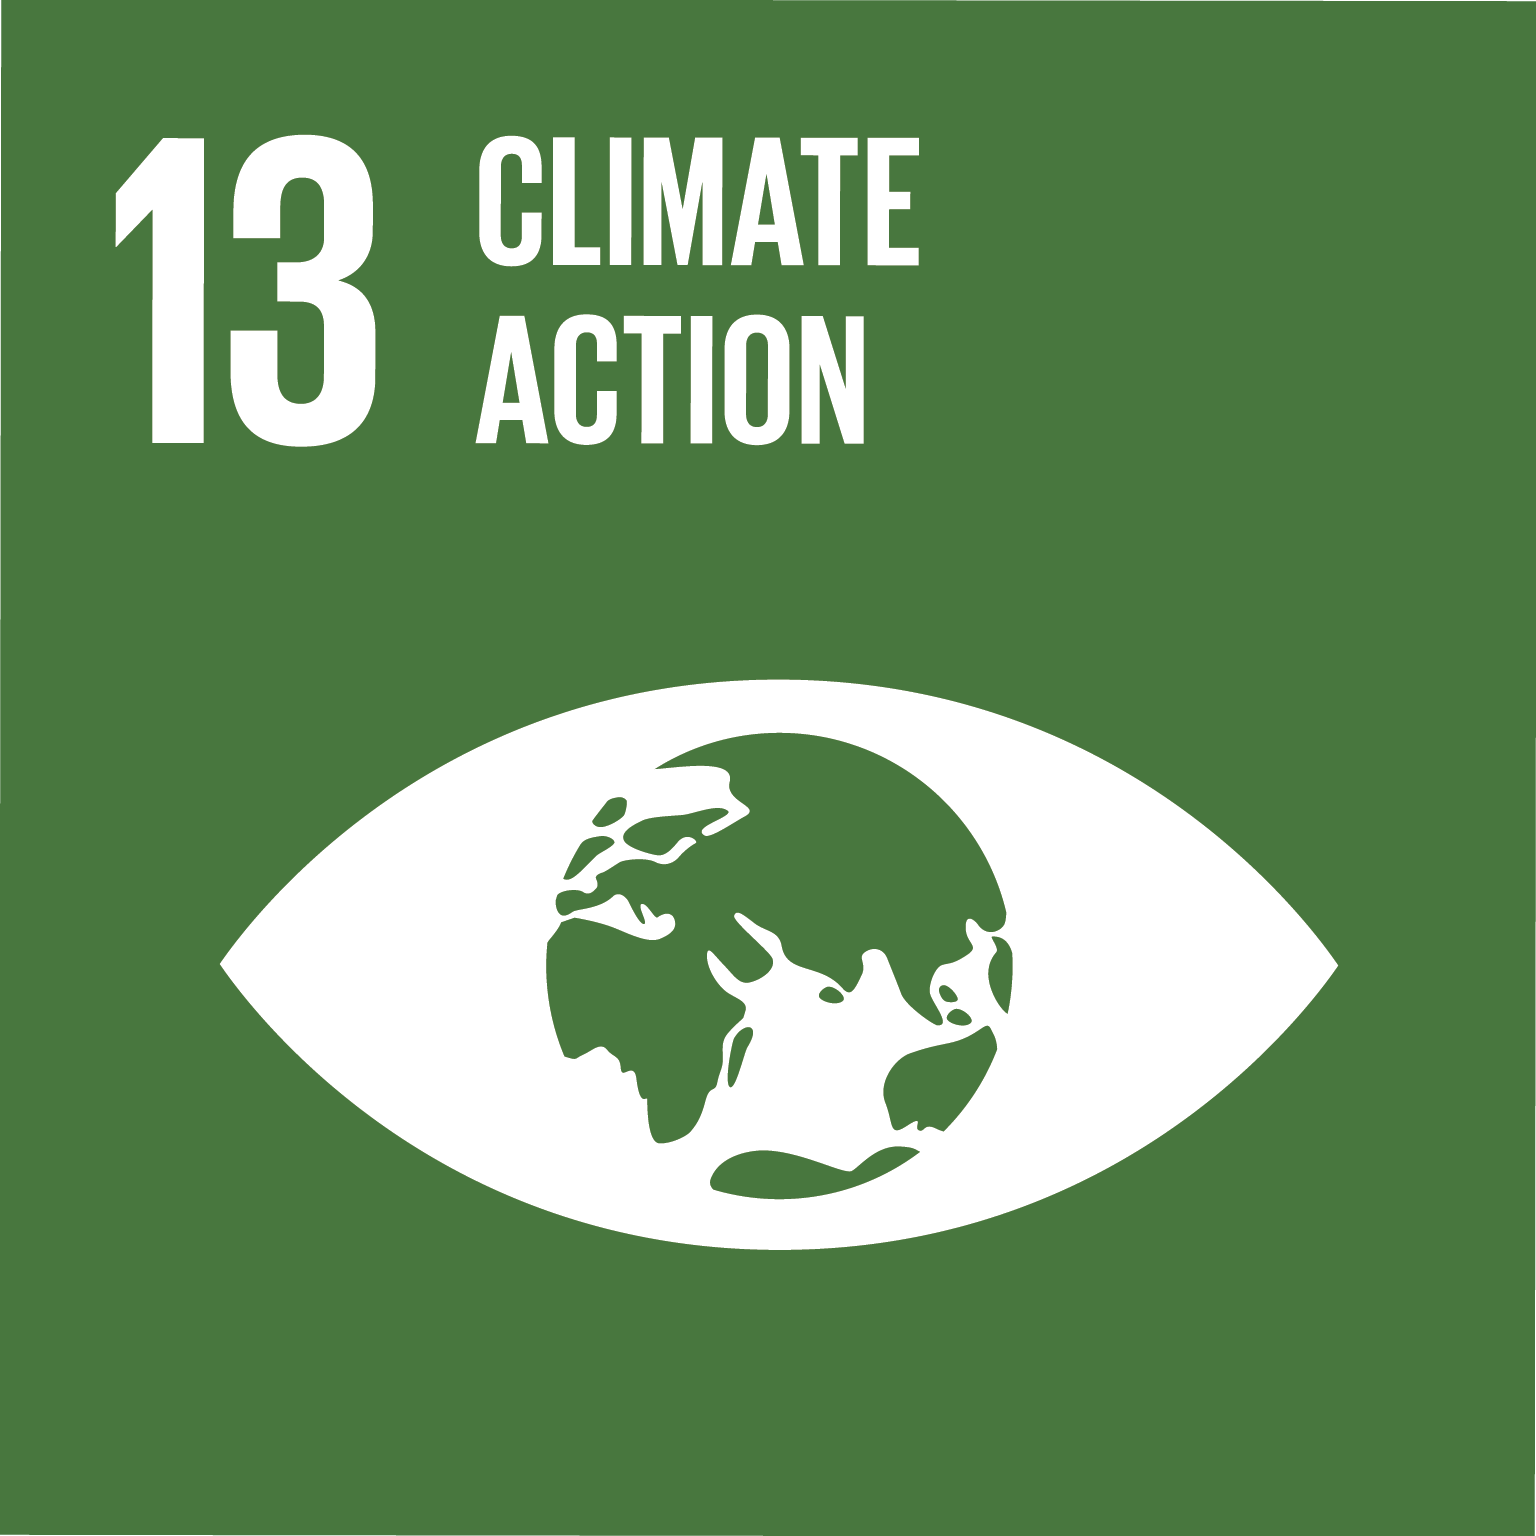
\includegraphics[height=4cm]{figures/sdg/sdg13.png}\hfill
    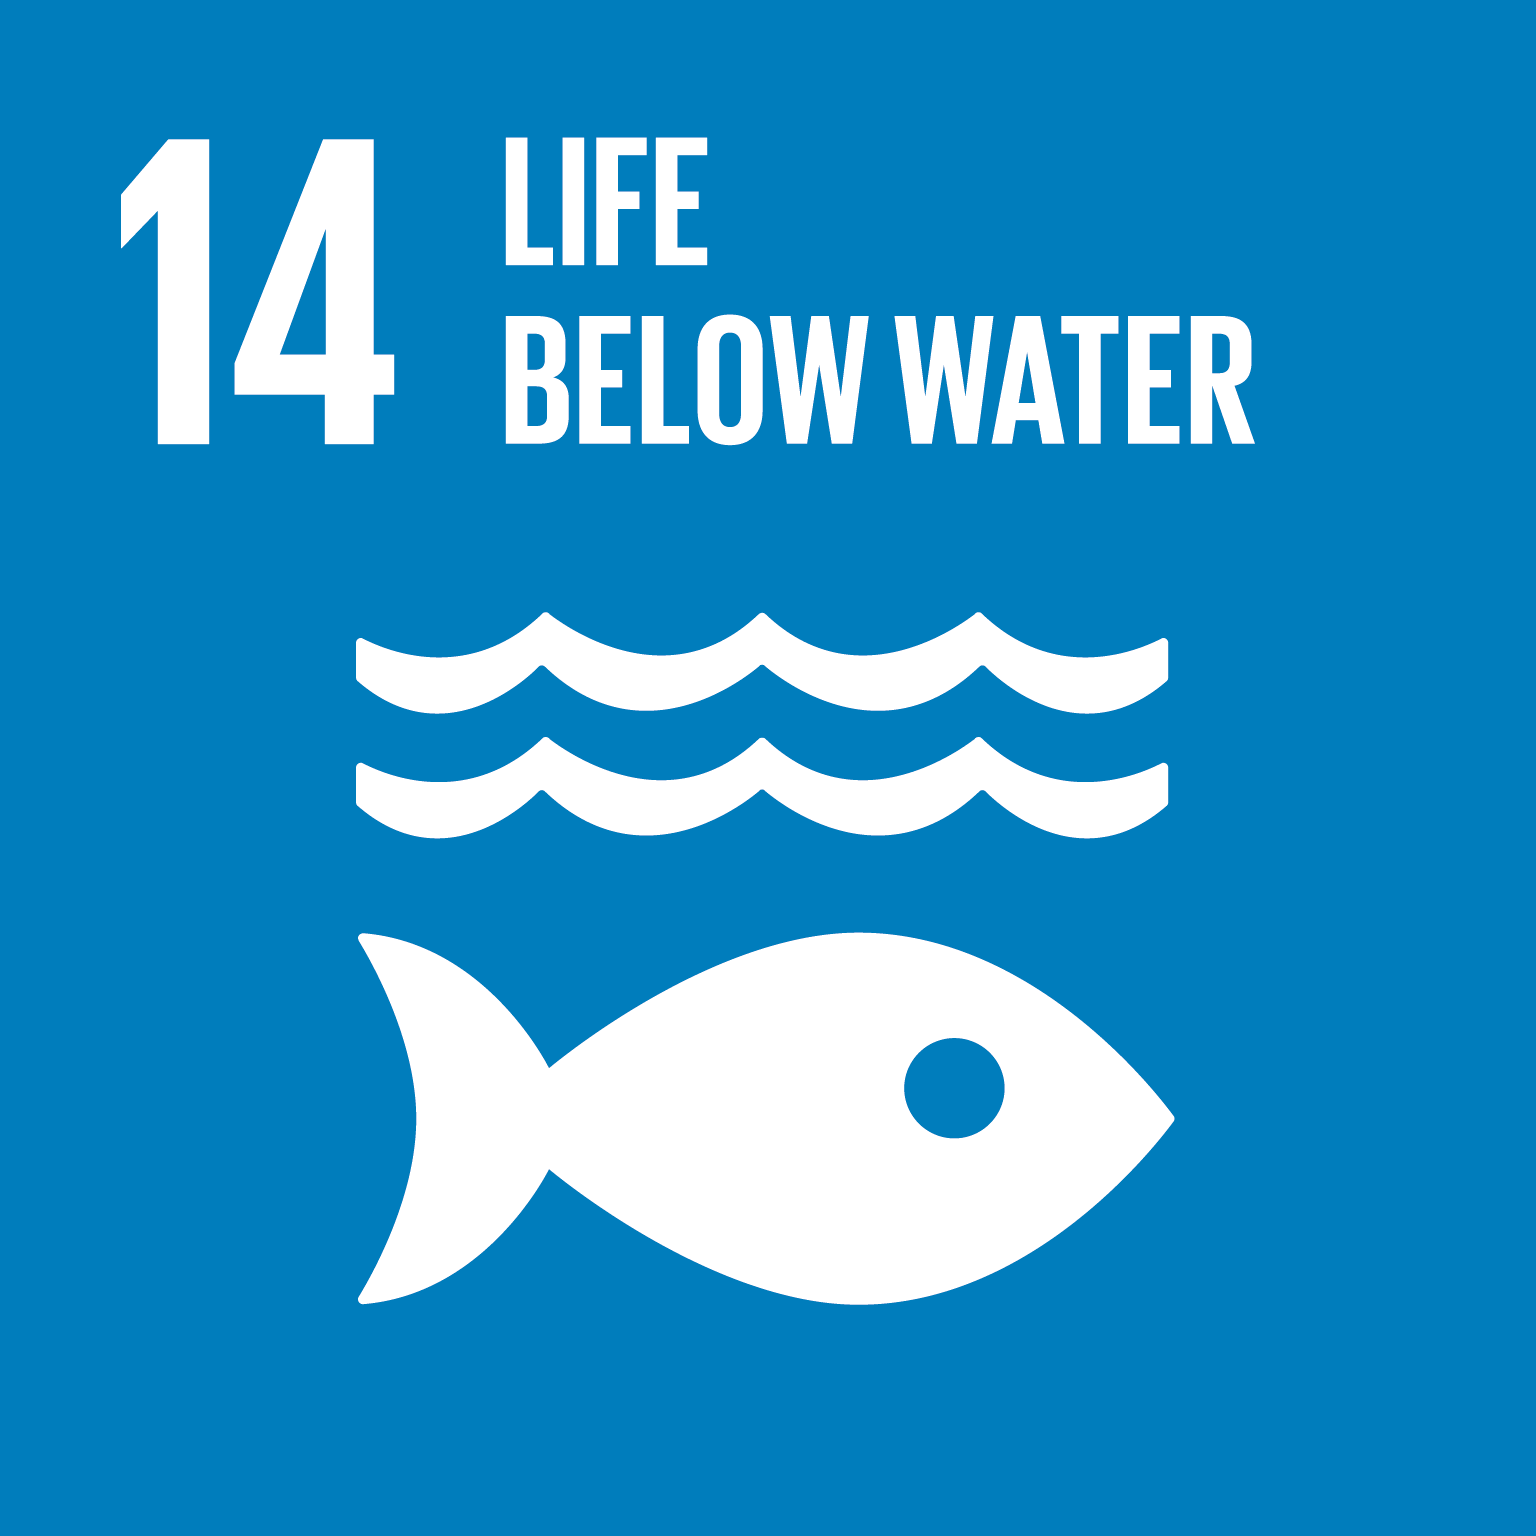
\includegraphics[height=4cm]{figures/sdg/sdg14.png}
    \caption[Sustainable Development Goals addressed by this thesis.]{\textbf{The
    three Sustainable Development Goals this thesis contributes to.} SDG~13
    (Climate Action), in particular target~13.3 on education, awareness and
    capacity; SDG~4 (Quality Education), on making complex knowledge accessible;
    and SDG~14 (Life Below Water), as the AMOC is part of the ocean system.
    Icons \textcopyright~United Nations. The content of this publication has not
    been approved by the United Nations and does not reflect its views.}
    \label{fig:sdg-alignment}
\end{figure}

% -------------------------------------------------------------------------
\section{Roadmap}
\label{sec:roadmap}

The thesis is organised around the detect--translate--evaluate arc, in three parts.

\textbf{Part~I --- DETECT} sets up the problem and delivers the analytical foundation the rest of the thesis builds on. Chapter~\ref{ch:rqs} formalises the research questions, objectives, hypotheses and design propositions. Chapter~\ref{ch:literature} reviews the literature, locates the thesis within it, and derives the design grammar that later governs every representational choice. Chapter~\ref{ch:background} develops the physical and mathematical apparatus needed to treat the AMOC as an analysable object. Chapter~\ref{ch:methodology} specifies the methodology governing all three phases and the standard of evidence each one answers to. Chapter~\ref{ch:data_pipeline} then carries out the analysis itself, reducing the AMOC's vertical structure to a compact, interpretable latent space, testing whether that reduction is faithful, and characterising the record's anomalies and early-warning behaviour.

\textbf{Part~II --- TRANSLATE} documents the constructive work. Chapter~\ref{ch:translate} designs the three representational conditions through which the recovered structure is made perceptible, states the commitments that keep the translation faithful, and presents the design grammar offered as this thesis's transferable contribution.

\textbf{Part~III --- EVALUATE} closes the loop and reflects on it. Chapter~\ref{ch:userstudy} specifies the user study and its instrument; Chapter~\ref{ch:results} reports what the coded responses show; Chapter~\ref{ch:discussion} interprets them and marks the boundaries of what they support; and Chapter~\ref{ch:conclusion} answers the research question, states the contribution and sets out what a larger study should do next. Chapter~\ref{ch:reflection} then steps outside the research to reflect on leadership, decision-making and personal growth across the project.

Three appendices carry the material the argument rests on but does not need in full. Appendix~\ref{app:ethics} consolidates the methodological boundaries, the limitations and the research ethics, including the use of AI assistants. Appendix~\ref{app:protocols} reproduces the study instruments and the coding grid against which the responses were analysed. And Appendix~\ref{app:code} documents the code, the computational environment and the provenance ledger that traces every perceivable element of the artefact back to its source in the data.
